\section{Continuous Random Variables}
\subsection{Basic definitions}
Recall that for a probability space $(\Omega,\mathscr F,\mathbb P)$, a random variable is a function $X:\Omega\to\mathbb R$ such that $\{X\le x\}=\{\omega\in\Omega:X(\omega)\le x\}\in\mathscr F$. 

\begin{definition}[Probability distribution function]
    The \textbf{probability distribution function} $ F:\bbR\to [0,1] $ is defined by $F(x)=\mathbb P(X\le x)$.
\end{definition}

\begin{proposition}\
    \begin{enumerate}
        \item $x\le y\implies F(x)\le F(y)$.
        \item $\forall a<b,\mathbb P(a<X\le b)=F(b)-F(a)$.
        \item $F$ is right continuous and the left limits always exist as well. Also,
        $$F(x-)=\mathbb{P}(X<x)\le F(x).$$
        \item $\displaystyle \lim_{x\to-\infty}F(x)=0,\lim_{x\to\infty}F(x)=1.$
    \end{enumerate}
\end{proposition}
\begin{proof}\
    \begin{enumerate}
        \item $ \{X\le x\} \subseteq \{X\le Y\} $.
        \item $ \mathbb{P}(a<x\le b)=\mathbb{P}(\{X>a\}\cap \{X\le b\})=\mathbb{P}(X\le b)-\mathbb{P}(\{X\le b\}\cap \{X\le a\})=\mathbb{P}(X\le b)-\mathbb{P}(X\le a)=F(b)-F(a) $.
        \item It suffices to prove $ \lim_{n \to \infty} F(x+\frac{1}{n})=F(x) $. Define $ A_n=\{x<X\le x+\frac{1}{n}\} $. Then $(A_n)$ are decreasing and $ \cap A_n = \varnothing $. But $ \mathbb{P}(A_n)=F(x+\frac{1}{n})-F(x)\to 0 $, so this proves right continuity. 

        Left limits exist since $F$ is increasing. Note that $ F(x-)=\lim_{n \to \infty} F(x-\frac{1}{n}) $ and that $ F(x-\frac{1}{n})=\mathbb{P}(X\le x-\frac{1}{n}) $. Consider $ B_n=\{X\le x-\frac{1}{n}\} $. Then $ (B_n) \nearrow, \cup B_n=\{X<x\} $, and $ \mathbb{P}(B_n)\to\mathbb{P}(X<x)\to F(x-)\le F(x) $.
        \item This one is easy.
    \end{enumerate}
\end{proof}

For example, $F$ of a discrete random variable might look like this:
\begin{center}
  \begin{tikzpicture}
    \draw [->] (0, 0) -- (3, 0);
    \draw [->] (0, 0) -- (0, 2) node [above] {$F$};
    \draw (0,0.5) -- (1,0.5);
    \node [dot=3.5pt] at (0,0.5) {};
    \draw [dashed] (1,0.5) -- (1,1);
    \node [dot=3.5pt] at (1,1) {};
    \node at (1,0.5) {$ \circ $};
    \draw (1,1) -- (2,1);
    \draw [dashed] (2,1) -- (2,1.5);
    \node [dot=3.5pt] at (2,1.5) {};
    \node at (2,1) {$ \circ $};
    \draw (2,1.5) -- (3,1.5);
    \node at (3,1.5) {$ \circ $};
  \end{tikzpicture}
\end{center}
It is indeed right continuous with left limits.

\begin{definition}[Continuous random variable]
    $X$ is a \textbf{continuous random variable} if $F$ is continuous, which means that $ F(x)=F(x-),\forall x \Longrightarrow \mathbb{P}(X\le x)=\mathbb{P}(X<x),\forall x $. In other words, $ \mathbb{P}(X=x)=0, \forall x\in \mathbb{R}  $.
    \begin{center}
        \begin{tikzpicture}
          \draw [->] (0, 0) -- (3, 0);
          \draw [->] (0, 0) -- (0, 2) node [above] {$F$};
          \draw (0, 0) parabola (2.5, 1.5);
        \end{tikzpicture}
    \end{center}
\end{definition}
\begin{definition}[Absolutely continous]
    $F$ is called \textbf{absolutely continous} if $F$ is not only continuous but also differentiable. 
\end{definition}
In this course we will further restrict to absolutely continuous $F$.

\subsection{Probability density function}

\begin{definition}[Probability density function]
    Set $F'(x)=f(x)$. We call $f$ the \textbf{probability density function} of $X$. 
\end{definition}

\begin{proposition}[Properties of $f$]\
    \begin{enumerate}
        \item$f(x)\ge 0$.
        \item $ \int_{-\infty}^x f(y)\,\mathrm dy=F(x). $ In particular, $ \int_{-\infty}^\infty f(y)\,\mathrm dy=1. $
    \end{enumerate}
\end{proposition}
Intuitively, for $\Delta x$ small, we have
\[
    \mathbb P(x<X\le x+\Delta x)=\int_x^{x+\Delta x}f(y)\,\mathrm dy\approx f(x)\Delta x,
\]
which is like approximating a continuous random variable by the probability density function of a discrete random variable. 

More generally, for any set $ S \subseteq \mathbb{R}  $, 
\[
    \mathbb{P}(x\in S) = \int_{S} f(x) \,\mathrm{d}x.
\]

\begin{center}
    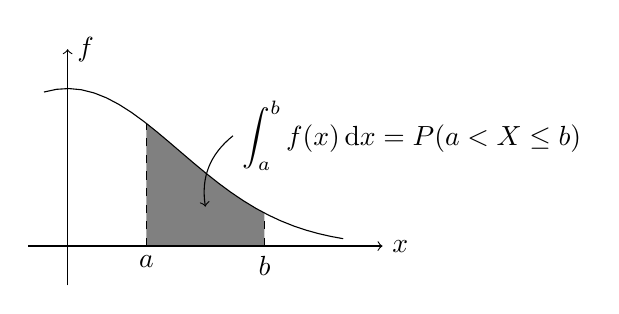
\begin{tikzpicture}
        \fill [gray, domain=1:2.5, variable=\x]
        (1, 0)
        -- plot (\x, {2 * exp(-\x * \x / 4)})
        -- (2.5, 0)
        -- cycle;
        \draw [->] (-0.5,0) -- (4,0) node [right] {$ x $};
        \draw [->] (0,-0.5) -- (0,2.5) node [right] {$ f $};
        \draw [domain=-0.3:3.5, variable=\x] plot (\x, {2 * exp(-\x * \x / 4)});
        \node [below] at (1,0) {$a$};
        \node [below] at (2.5,0) {$b$};
        \draw [->, bend right] (2.1, 1.4) to (1.75, 0.5);
        \node [right] at (2.1, 1.4) {$\displaystyle \int_{a}^{b} f(x) \,\mathrm{d}x = \mathbb{P}(a<X\le b)$};
        \draw [dashed] (1,0) -- (1,1.56);
        \draw [dashed] (2.5,0) -- (2.5,0.42);
    \end{tikzpicture}
\end{center}